% This must be in the first 5 lines to tell arXiv to use pdfLaTeX, which is strongly recommended.
\pdfoutput=1
% In particular, the hyperref package requires pdfLaTeX in order to break URLs across lines.

\documentclass[11pt]{article}
\usepackage{graphicx}


% Remove the "review" option to generate the final version.
\usepackage[review]{ACL2023}

% Standard package includes
\usepackage{times}
\usepackage{latexsym}

% For proper rendering and hyphenation of words containing Latin characters (including in bib files)
\usepackage[T1]{fontenc}
% For Vietnamese characters
% \usepackage[T5]{fontenc}
% See https://www.latex-project.org/help/documentation/encguide.pdf for other character sets

% This assumes your files are encoded as UTF8
\usepackage[utf8]{inputenc}

% This is not strictly necessary, and may be commented out.
% However, it will improve the layout of the manuscript,
% and will typically save some space.
\usepackage{microtype}

% This is also not strictly necessary, and may be commented out.
% However, it will improve the aesthetics of text in
% the typewriter font.
\usepackage{inconsolata}


% If the title and author information does not fit in the area allocated, uncomment the following
%
%\setlength\titlebox{<dim>}
%
% and set <dim> to something 5cm or larger.

\title{RL-LLM Paper}


\author{First Author \\
  Affiliation / Address line 1 \\
  Affiliation / Address line 2 \\
  Affiliation / Address line 3 \\
  \texttt{email@domain} \\\And
  Second Author \\
  Affiliation / Address line 1 \\
  Affiliation / Address line 2 \\
  Affiliation / Address line 3 \\
  \texttt{email@domain} \\}

\begin{document}
\maketitle
\begin{abstract}
As the use of LLMs is growing more common for a wide array of domains, understanding their behavior in order to harness their capacity is essential to ensure that they can provide a meaningful contribution to the task at hand. In this paper, we examine the issue of calibration by replicating elements of Kadavath 2022's study, focusing on the Humaneval and GSM datasets and experimenting with few shot prompting and different prompt formats, specifically on the 7B base and chat LLama models. By evaluating the model on True/False prompts and prompting it with both 0-shot and 5-shot methods, we find that few-shot prompting does indeed result in better-calibrated outputs. We also provide the model with prompts in which they are required to choose from several answers, along with a none of the above option.
\end{abstract}



\section{Introduction}

Beyond producing grammatically sound input, LLMs need to provide the user with information that correctly reflects the reality of the world, i.e the ground truth. Sometimes, the model might not have access to or may not identify the ground truth correctly, resulting in fluent, but factually incorrect output, named 'hallucinations'. Ideally, we want the model itself to be aware of how its own output relates to the ground truth value. An example of such a measure is calibration. Calibration refers to the interaction between the confidence of a prediction and its empirical likelihood. In the case of a perfectly calibrated model, the relationship is linear (SOURCE). 
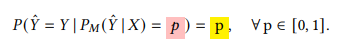
\includegraphics{figures/calibration_formula.PNG}

Several observations have been made on the topic of calibration in LLMs specifically. (SOURCE PAPER) finds that the probabilities assigned to answer options on benchmark datasets seem to correlate with correctness probabilities, a tendency which is especially visible for the results obtained by bigger models (SOURCE). They also mention that while LLMs are generally well-calibrated, the use of reinforcement learning can sometimes damage calibration, but that a temperature adjustement seems to do the trick in replacing the model on the path of correct calibration
In this study, we aim to replicate the findings of (SOURCE)

\section{Methods}
\subsection{Models}



\section{Results}


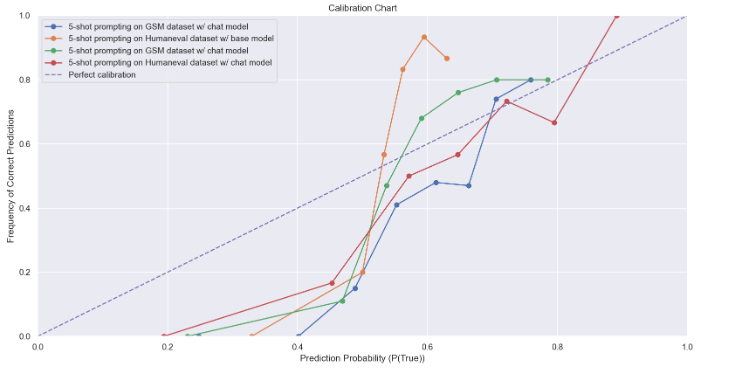
\includegraphics[0.25]{figures/5shot.PNG}
\includegraphics[0.25]{figures/zeroshot.PNG}
\newpage
\pagebreak

% Entries for the entire Anthology, followed by custom entries
\bibliography{custom}
\bibliographystyle{acl_natbib}

\appendix

\section{Example Appendix}
\label{sec:appendix}

This is a section in the appendix.

\end{document}
